% Options for packages loaded elsewhere
\PassOptionsToPackage{unicode}{hyperref}
\PassOptionsToPackage{hyphens}{url}
%
\documentclass[
  a4paper,
]{article}
\usepackage{amsmath,amssymb}
\usepackage{setspace}
\usepackage{iftex}
\ifPDFTeX
  \usepackage[T1]{fontenc}
  \usepackage[utf8]{inputenc}
  \usepackage{textcomp} % provide euro and other symbols
\else % if luatex or xetex
  \usepackage{unicode-math} % this also loads fontspec
  \defaultfontfeatures{Scale=MatchLowercase}
  \defaultfontfeatures[\rmfamily]{Ligatures=TeX,Scale=1}
\fi
\usepackage{lmodern}
\ifPDFTeX\else
  % xetex/luatex font selection
\fi
% Use upquote if available, for straight quotes in verbatim environments
\IfFileExists{upquote.sty}{\usepackage{upquote}}{}
\IfFileExists{microtype.sty}{% use microtype if available
  \usepackage[]{microtype}
  \UseMicrotypeSet[protrusion]{basicmath} % disable protrusion for tt fonts
}{}
\makeatletter
\@ifundefined{KOMAClassName}{% if non-KOMA class
  \IfFileExists{parskip.sty}{%
    \usepackage{parskip}
  }{% else
    \setlength{\parindent}{0pt}
    \setlength{\parskip}{6pt plus 2pt minus 1pt}}
}{% if KOMA class
  \KOMAoptions{parskip=half}}
\makeatother
\usepackage{xcolor}
\usepackage[margin=1in]{geometry}
\usepackage{graphicx}
\makeatletter
\def\maxwidth{\ifdim\Gin@nat@width>\linewidth\linewidth\else\Gin@nat@width\fi}
\def\maxheight{\ifdim\Gin@nat@height>\textheight\textheight\else\Gin@nat@height\fi}
\makeatother
% Scale images if necessary, so that they will not overflow the page
% margins by default, and it is still possible to overwrite the defaults
% using explicit options in \includegraphics[width, height, ...]{}
\setkeys{Gin}{width=\maxwidth,height=\maxheight,keepaspectratio}
% Set default figure placement to htbp
\makeatletter
\def\fps@figure{htbp}
\makeatother
\setlength{\emergencystretch}{3em} % prevent overfull lines
\providecommand{\tightlist}{%
  \setlength{\itemsep}{0pt}\setlength{\parskip}{0pt}}
\setcounter{secnumdepth}{-\maxdimen} % remove section numbering
\ifLuaTeX
\usepackage[bidi=basic]{babel}
\else
\usepackage[bidi=default]{babel}
\fi
\babelprovide[main,import]{catalan}
% get rid of language-specific shorthands (see #6817):
\let\LanguageShortHands\languageshorthands
\def\languageshorthands#1{}
\ifLuaTeX
  \usepackage{selnolig}  % disable illegal ligatures
\fi
\usepackage{bookmark}
\IfFileExists{xurl.sty}{\usepackage{xurl}}{} % add URL line breaks if available
\urlstyle{same}
\hypersetup{
  pdftitle={GUIA RÀPIDA ``ECOSIA.ORG''},
  pdfauthor={@tofermos 2025},
  pdflang={ca-ES},
  hidelinks,
  pdfcreator={LaTeX via pandoc}}

\title{GUIA RÀPIDA ``ECOSIA.ORG''}
\usepackage{etoolbox}
\makeatletter
\providecommand{\subtitle}[1]{% add subtitle to \maketitle
  \apptocmd{\@title}{\par {\large #1 \par}}{}{}
}
\makeatother
\subtitle{Caràcterístiques d'Ecosia i configuració per l'ús en Firefox,
Chrome i Edge}
\author{@tofermos 2025}
\date{}

\begin{document}
\maketitle

{
\setcounter{tocdepth}{2}
\tableofcontents
}
\setstretch{1.5}
\newpage
\renewcommand\tablename{Tabla}

\section{1 🌱 El per què d'usar
Ecosia}\label{el-per-quuxe8-dusar-ecosia}

Ecosia és un \textbf{motor de cerca} que utilitza els ingressos
publicitaris per finançar la plantació d'arbres arreu del món. Funciona
de manera similar a Google, però està fortament enfocat en la
\textbf{sostenibilitat i la privacitat} dels usuaris.

\subsection{1.1 Per raons mediamientals}\label{per-raons-mediamientals}

L'aposta per la sostenibilitat i l'impacte positiu en el medi ambient
d'este motor es pot detallar en els següents punts:

\subsubsection{Plantació d'arbres}\label{plantaciuxf3-darbres}

\begin{itemize}
\tightlist
\item
  Ecosia destina els seus beneficis a la plantació d'arbres arreu del
  món. Aproximadament cada 45 cerques generen suficients ingressos per
  plantar un arbre.
\end{itemize}

\subsubsection{Ús d'energies
renovables}\label{uxfas-denergies-renovables}

\begin{itemize}
\tightlist
\item
  Ecosia utilitza el 100\% dels seus ingressos publicitaris per finançar
  projectes verds i sostenibles.
\item
  Els seus servidors funcionen amb energia renovable. Fins i tot
  produeixen més electricitat neta de la que consumeixen.
\end{itemize}

\subsubsection{Reducció de la petjada de
carboni}\label{reducciuxf3-de-la-petjada-de-carboni}

\begin{itemize}
\tightlist
\item
  Mentre Ecosia treballa activament per compensar les emissions de CO₂,
  Google, per exemple té una gran petjada de carboni.
\end{itemize}

\subsection{1.2 Per raons ètiques}\label{per-raons-uxe8tiques}

\subsubsection{Privadesa i protecció de dades personals o
organitzacionals}\label{privadesa-i-protecciuxf3-de-dades-personals-o-organitzacionals}

\begin{itemize}
\tightlist
\item
  No emmagatzema cerques de manera permanent.
\item
  No ven dades a anunciants ni utilitza eines de seguiment invasives.
\item
  Les búsquedes són encriptades per protegir la privadesa dels usuaris.
\end{itemize}

\subsubsection{Transparència
financera}\label{transparuxe8ncia-financera}

\begin{itemize}
\tightlist
\item
  Ecosia publica informes mensuals sobre els seus ingressos i com es
  distribueixen els diners, cosa que ofereix més transparència que
  Google.
\end{itemize}

\href{https://ecosia.helpscoutdocs.com/article/402-reports-transparency}{Informes
financers}

\subsubsection{Suport a comunitats
locals}\label{suport-a-comunitats-locals}

\begin{itemize}
\tightlist
\item
  Els projectes de reforestació d'Ecosia tenen un impacte directe en
  comunitats afectades per la desforestació, ajudant a crear llocs de
  treball i restaurar ecosistemes.
\end{itemize}

\newpage

\section{2 🔧 Configuració en
navegadors}\label{configuraciuxf3-en-navegadors}

Quan usem el buscador www.ecosia.org, el navegador usa el motor de
búsqueda de ecosia idependentment del que tinguem configurat al
navegador. Per a això establirem esta pàgina com la d'inici per defecte.

Independentment, configurarem el motor d'Ecosia per defecte al navegador
ecara que hem de saber que si usem www.google.com, s'usará el motor de
de google no el d'ecosia.

\subsection{2.1 Navegador Firefox}\label{navegador-firefox}

Entrem la configuració del navegador

\begin{figure}
\centering
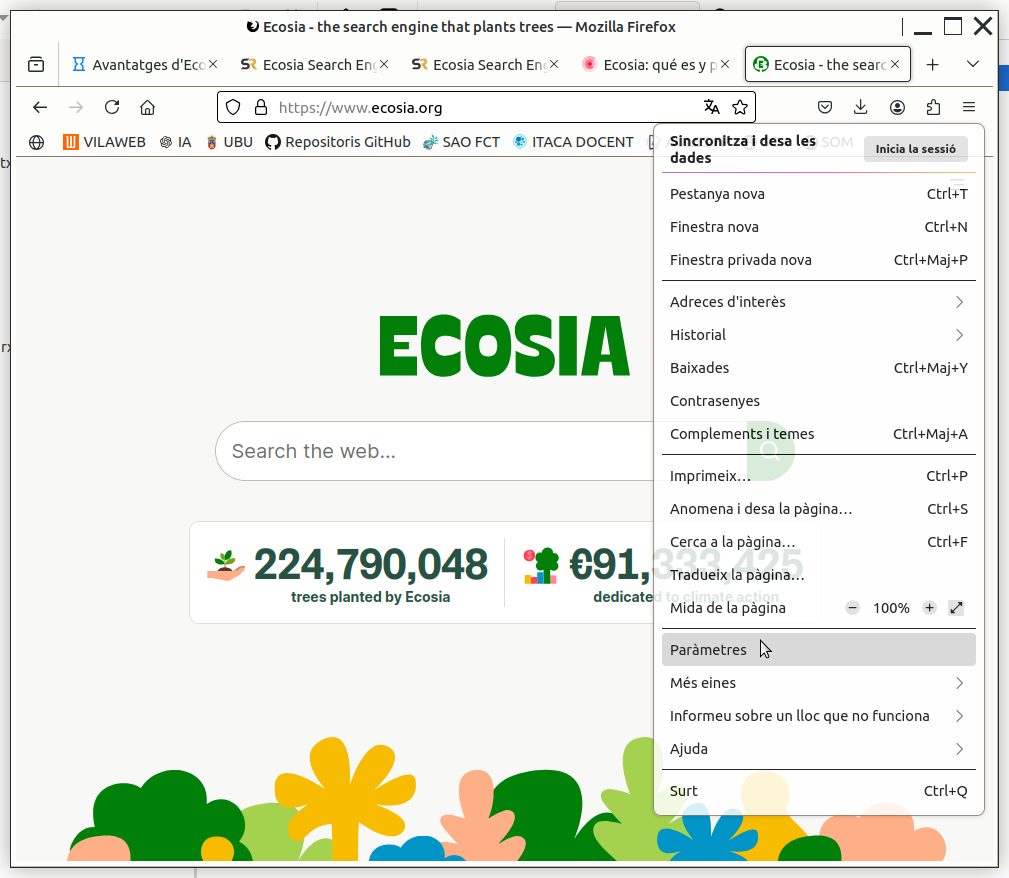
\includegraphics{png/1-Firefox-Parametres.png}
\caption{\emph{Imatge 1: Opció paràmatres de Firefox}}
\end{figure}

\begin{center}\rule{0.5\linewidth}{0.5pt}\end{center}

\subsubsection{Motor de cerca
predeterminat}\label{motor-de-cerca-predeterminat}

Una vegada estem en la configuració del navegador, busquem ``motor'' i
seleccionem el que volem: ecosia.

\begin{figure}
\centering
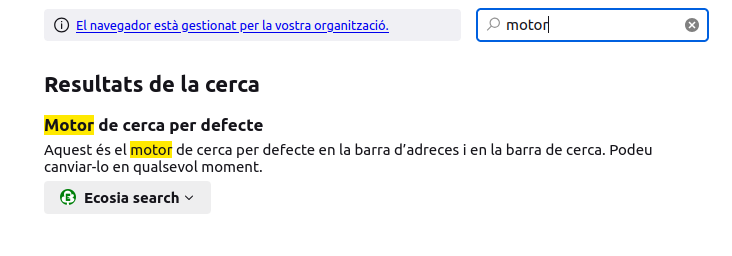
\includegraphics{png/2-Firefox-Motor.png}
\caption{\emph{Imatge 2: Motor de búsqueda en Firefox}}
\end{figure}

\begin{center}\rule{0.5\linewidth}{0.5pt}\end{center}

\subsubsection{Pàgina d'inici}\label{puxe0gina-dinici}

Per fer ús del buscador còmodament, a banda del motor, podem canviar la
pàgina d'inici predeterminada.

Des de l mateixa configuració (``paràmetres''), busquem ``Inici'' i
escrivim la pàgina de ecosia.org

\begin{figure}
\centering
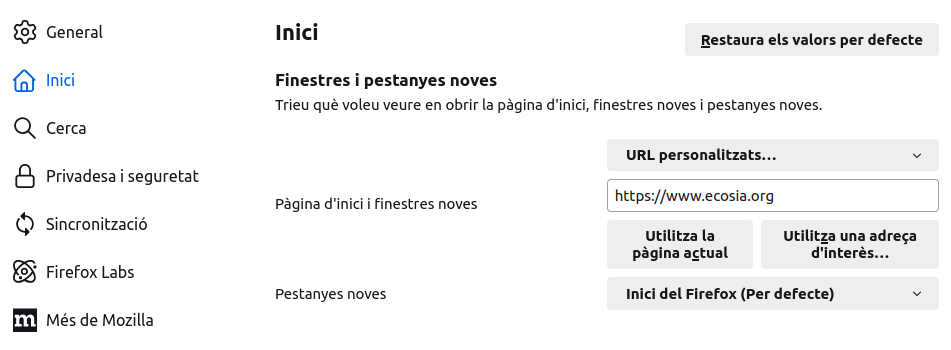
\includegraphics{png/3-Firefox-Inici.png}
\caption{\emph{Imatge 3: Pàgina d'inici en Firefox}}
\end{figure}

\begin{center}\rule{0.5\linewidth}{0.5pt}\end{center}

\subsection{2.2 Navegador Chrome}\label{navegador-chrome}

Entrem la configuració del navegador

\begin{figure}
\centering
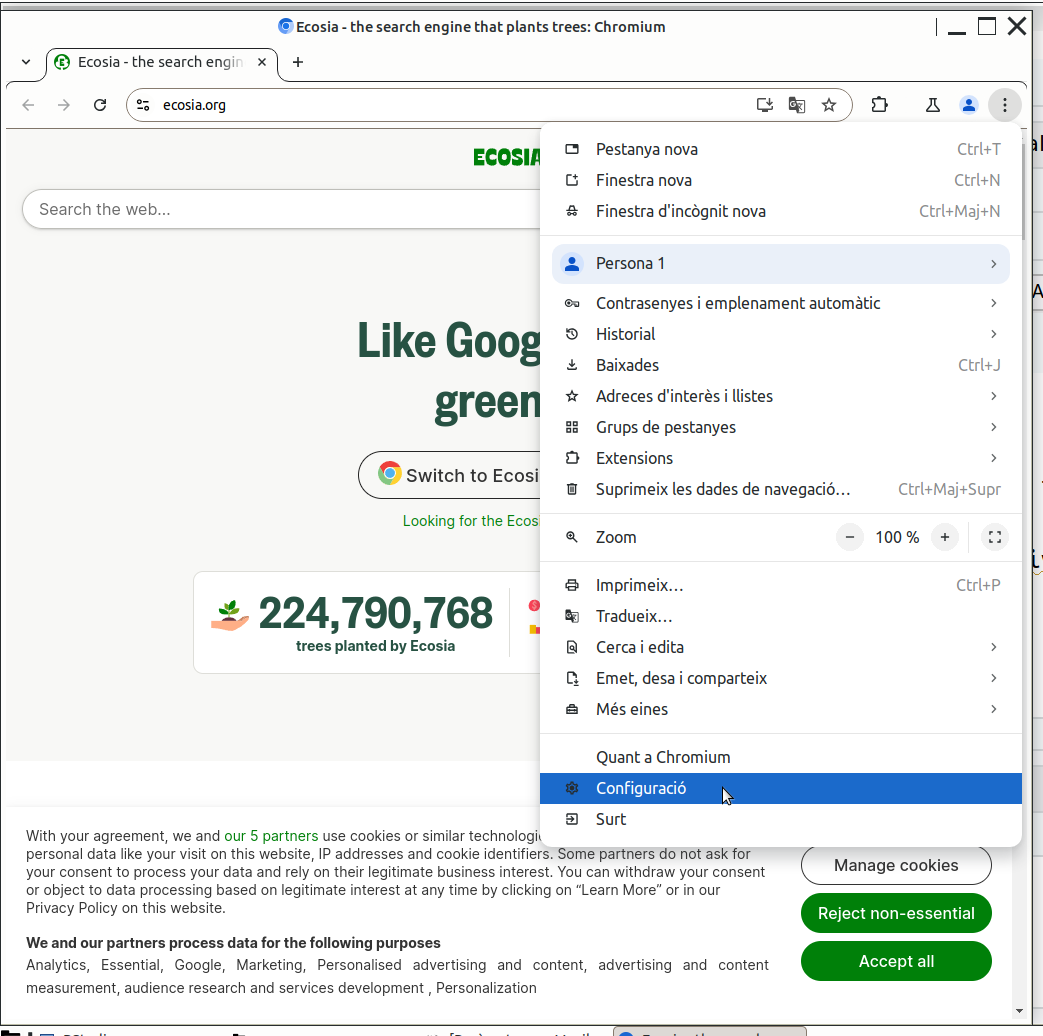
\includegraphics{png/1-Chrome-Configuracio.png}
\caption{\emph{Imatge 4: Opció configuració de Chrome}}
\end{figure}

\begin{center}\rule{0.5\linewidth}{0.5pt}\end{center}

\subsubsection{Motor de cerca
predeterminat}\label{motor-de-cerca-predeterminat-1}

Una vegada estem en la configuració del navegador, busquem ``motor'' i
seleccionem el que volem: ecosia.

\begin{figure}
\centering
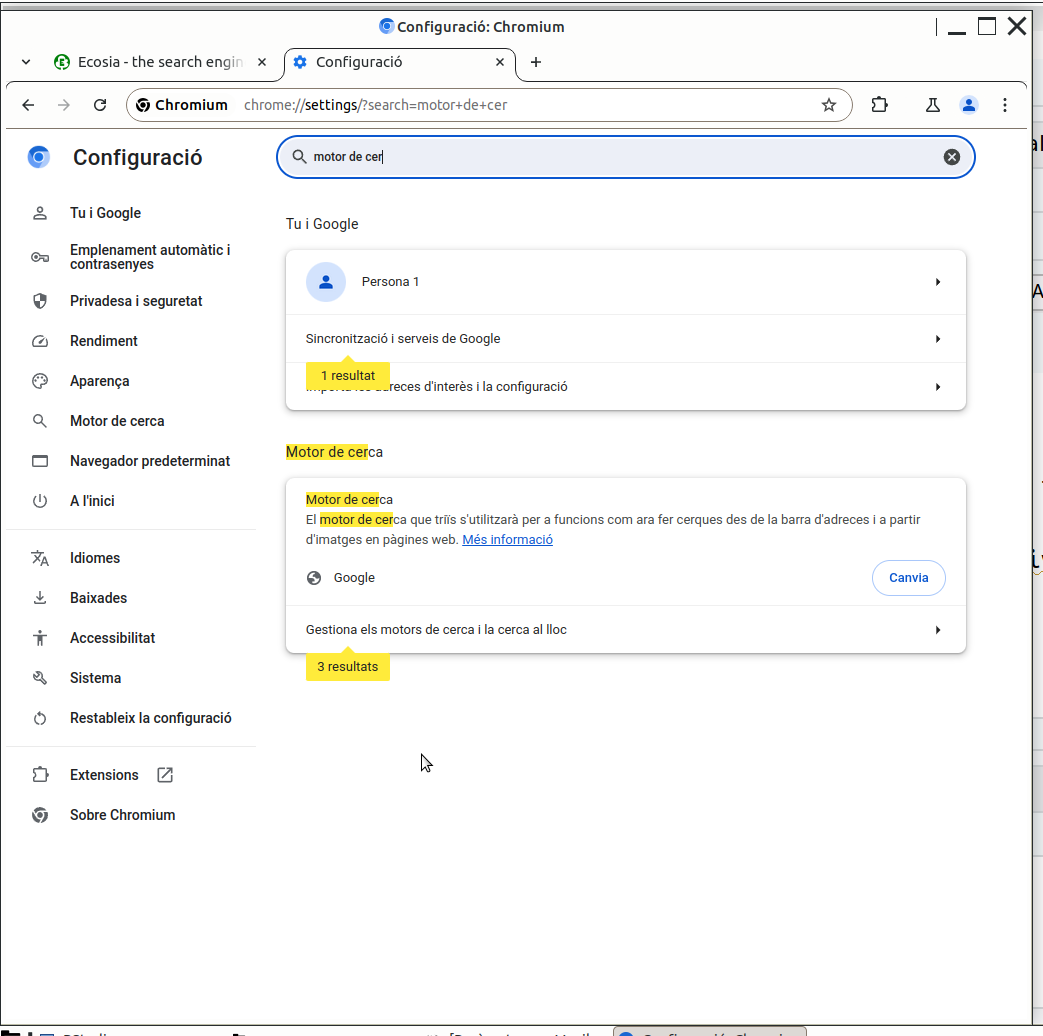
\includegraphics{png/2-Chrome-Motor.png}
\caption{\emph{Imatge 5: Motor de búsqueda en Chrome}}
\end{figure}

\begin{center}\rule{0.5\linewidth}{0.5pt}\end{center}

\subsubsection{Pàgina d'inici}\label{puxe0gina-dinici-1}

Per fer ús del buscador còmodament, a banda del motor, podem canviar la
pàgina d'inici predeterminada.

Des de l mateixa configuració, seleccionem ``Inici'' i escrivim la
pàgina de ecosia.org

\begin{figure}
\centering
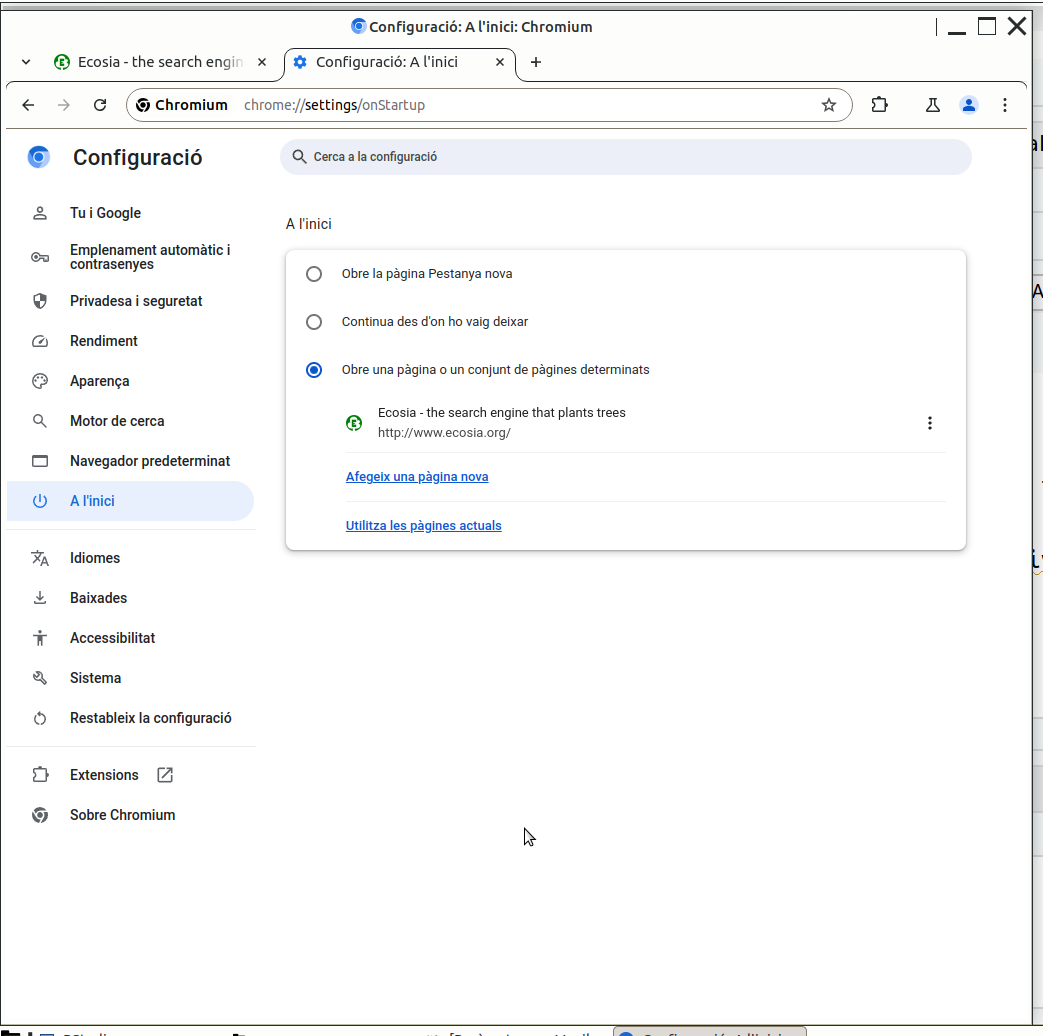
\includegraphics{png/3-Chrome-Inici.png}
\caption{\emph{Imatge 6 Pàgina d'inici en Chrome}}
\end{figure}

\begin{center}\rule{0.5\linewidth}{0.5pt}\end{center}

\subsection{2.3 Navegador Edge (MS
Windows)}\label{navegador-edge-ms-windows}

Punxem en els \textbf{···} i seleccionem \textbf{Configuració}

\begin{figure}
\centering
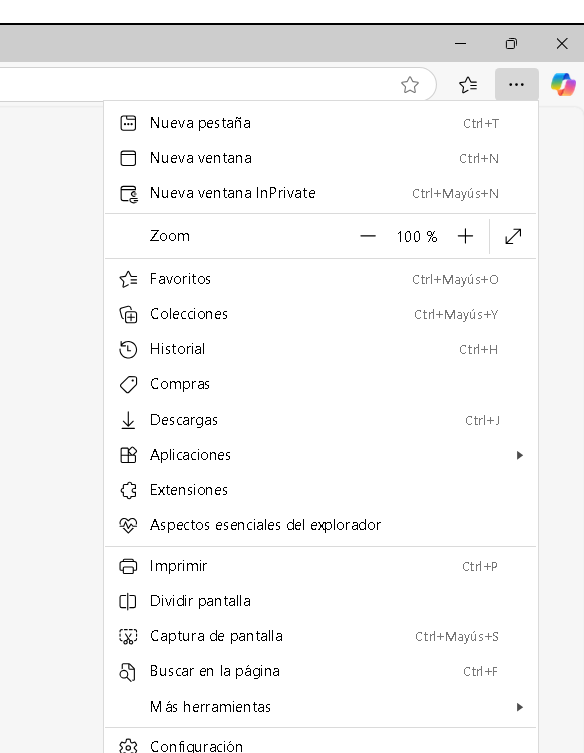
\includegraphics{png/0-EdgeConfiguracio.png}
\caption{\emph{Imatge 7: Configuració de Edge}}
\end{figure}

\begin{center}\rule{0.5\linewidth}{0.5pt}\end{center}

\subsubsection{Motor de cerca
predeterminat}\label{motor-de-cerca-predeterminat-2}

\begin{figure}
\centering
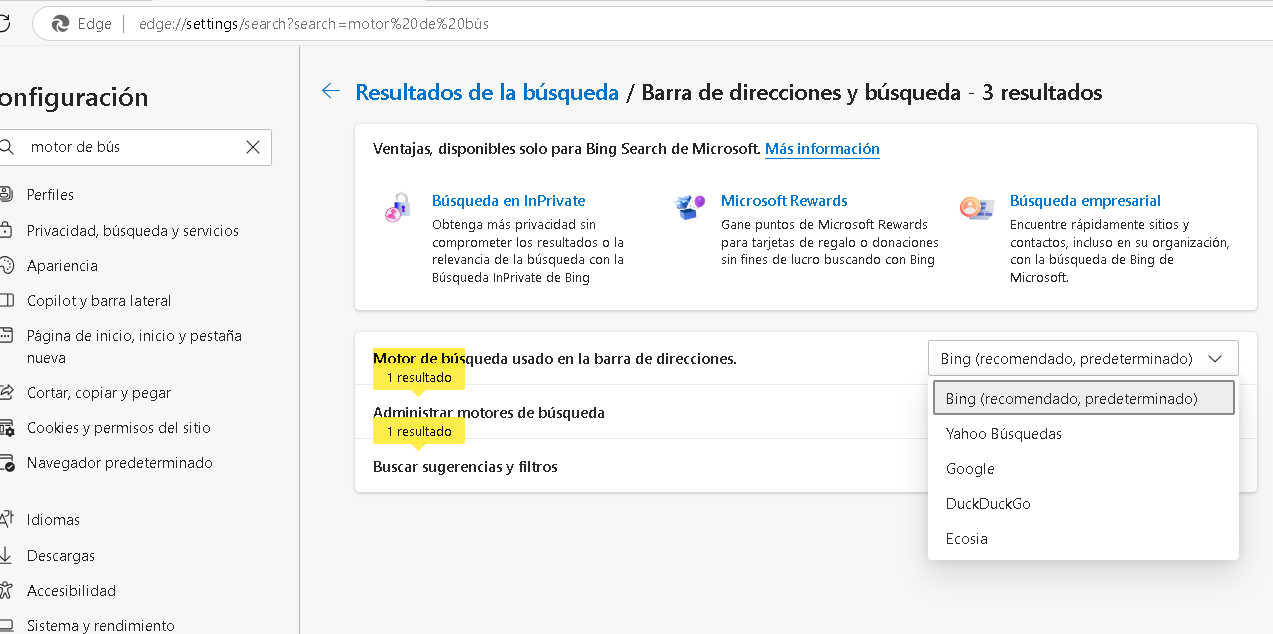
\includegraphics{png/1-EdgeMotor.png}
\caption{\emph{Imatge 8: Motor de cerca Ecosia en Edge}}
\end{figure}

\subsubsection{Pàgina d'inici}\label{puxe0gina-dinici-2}

\begin{figure}
\centering
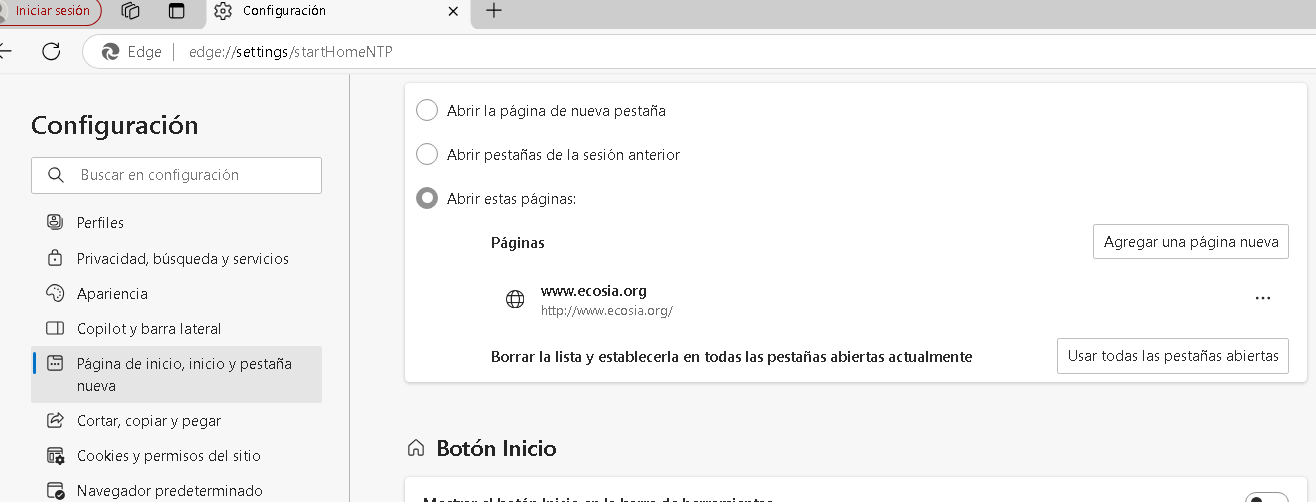
\includegraphics{png/2-EdgeInici.png}
\caption{\emph{Imatge 9: Pàgina d'inici}}
\end{figure}

\begin{center}\rule{0.5\linewidth}{0.5pt}\end{center}

\newpage

\section{3 🧩 Extensió d'Ecosia}\label{extensiuxf3-decosia}

La extensió \textbf{NO és necessària} per treballar amb Ecosia però
ofereix:

\begin{itemize}
\tightlist
\item
  Comptador d'arbres plantats.
\item
  Configuració més ràpida i fàcil.
\item
  Bloqueig de rastrejadors per més privacitat.
\end{itemize}

\subsection{3.1 Extensions en Firefox}\label{extensions-en-firefox}

\begin{figure}
\centering
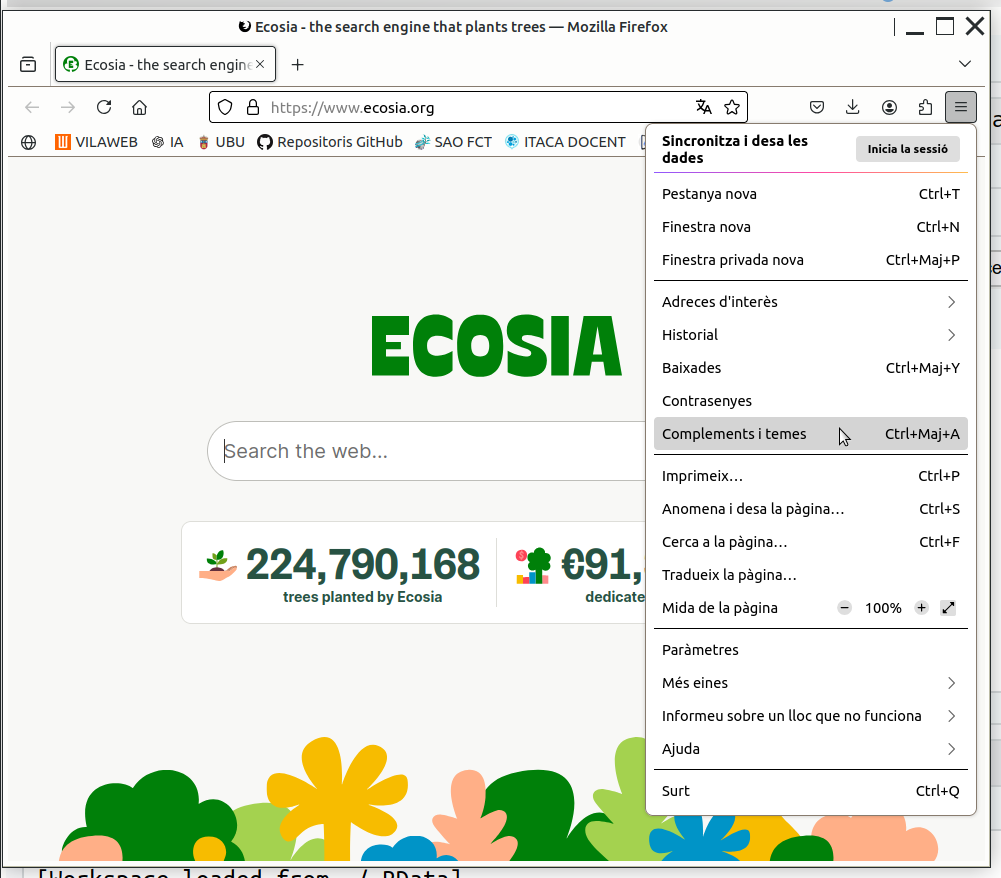
\includegraphics{png/0-ExtensionsFirefox.png}
\caption{\emph{Imatge 10: Selecciona opció Complements i temes}}
\end{figure}

\begin{center}\rule{0.5\linewidth}{0.5pt}\end{center}

\begin{figure}
\centering
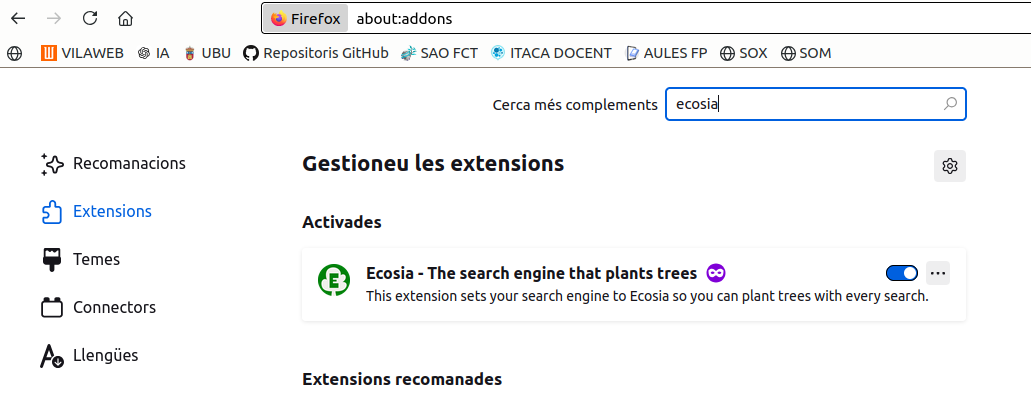
\includegraphics{png/1-ExtensionsFirefox.png}
\caption{\emph{Imatge 11: Buscar l'extensió}}
\end{figure}

\begin{center}\rule{0.5\linewidth}{0.5pt}\end{center}

\subsection{3.2 Extensions en Chrome}\label{extensions-en-chrome}

Entrem en \textbf{···} i seleccionem \textbf{Extensions}.

\begin{figure}
\centering
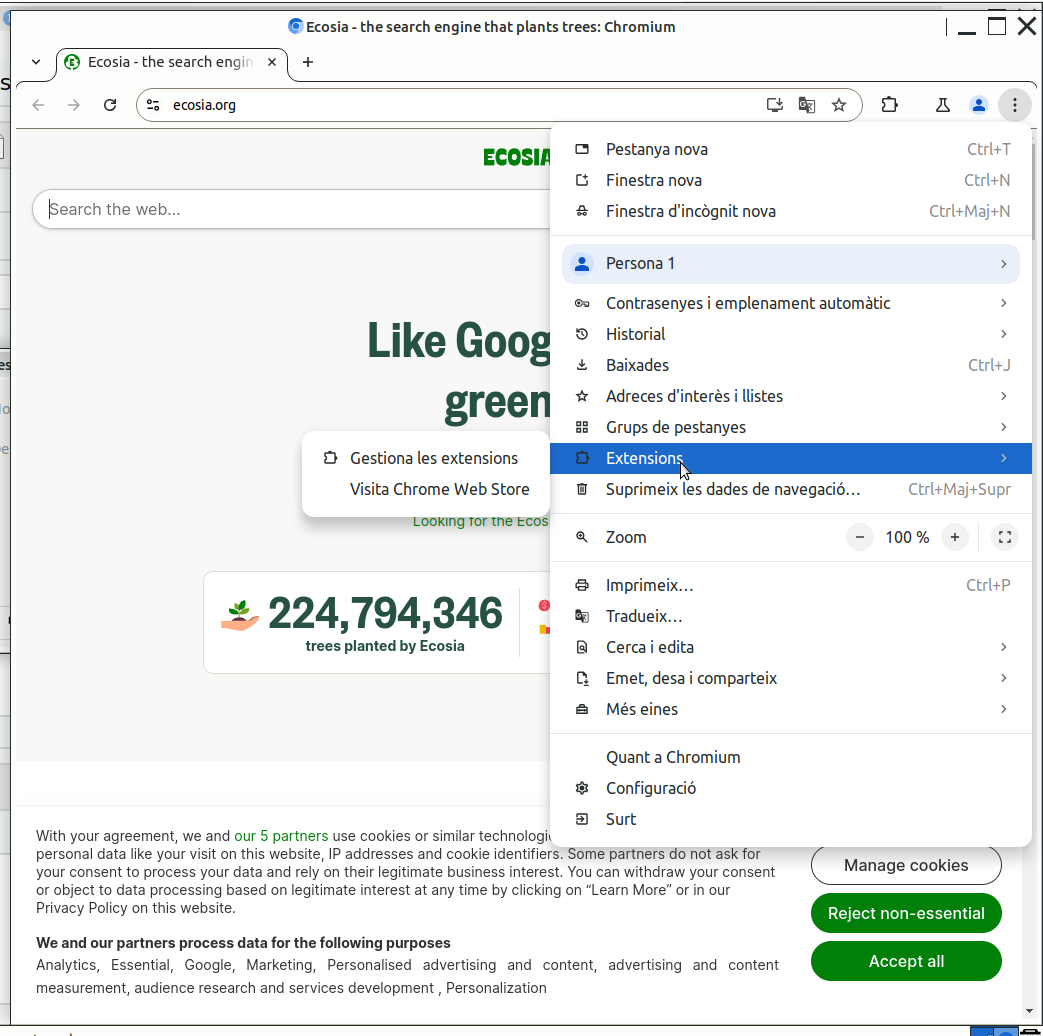
\includegraphics{png/1-ChromeExtensions.png}
\caption{\emph{Imatge 12: Selecciona Extensions}}
\end{figure}

\begin{center}\rule{0.5\linewidth}{0.5pt}\end{center}

\begin{figure}
\centering
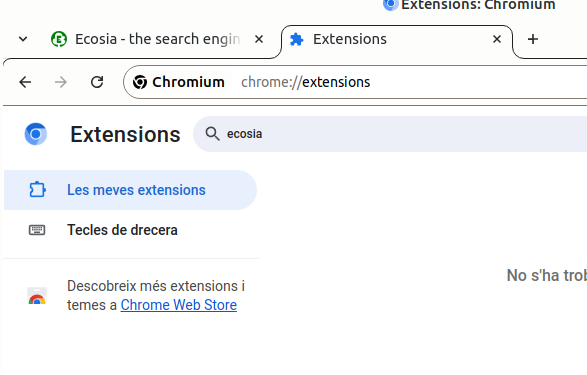
\includegraphics{png/2-ChromeExtensions.png}
\caption{\emph{Imatge 13: Selecciona Chrome Web Store}}
\end{figure}

\begin{center}\rule{0.5\linewidth}{0.5pt}\end{center}

\begin{figure}
\centering
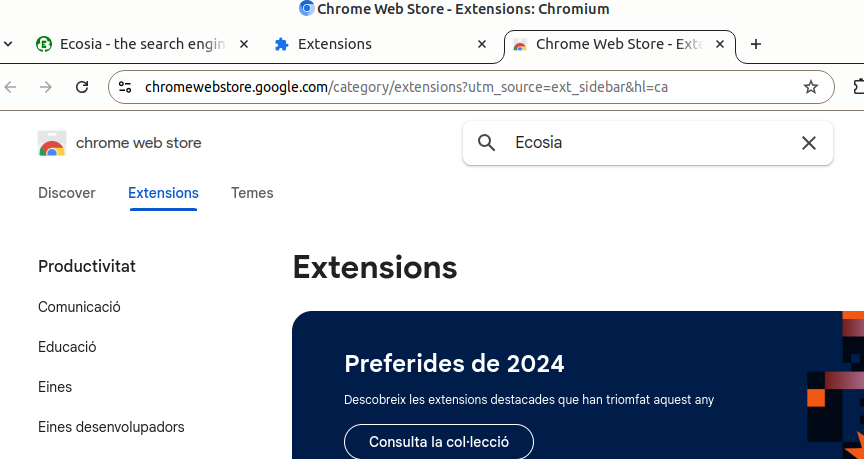
\includegraphics{png/3-ChromeExtensions.png}
\caption{\emph{Imatge 14: Busca i instal·la l'extensió}}
\end{figure}

\begin{center}\rule{0.5\linewidth}{0.5pt}\end{center}

\subsection{3.2 Extensions en Edge}\label{extensions-en-edge}

Entrem en \textbf{···} i seleccionem \textbf{Configuración}. Després
\textbf{Obtenir extensions per a MS Edge}

\begin{figure}
\centering
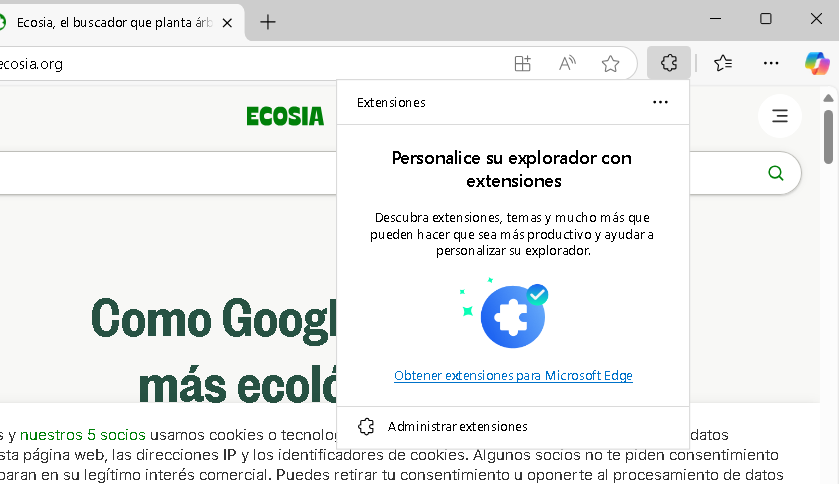
\includegraphics{png/0-EdgeExtensions.png}
\caption{\emph{Imatge 15: Extensions de Edge}}
\end{figure}

\begin{center}\rule{0.5\linewidth}{0.5pt}\end{center}

\begin{figure}
\centering
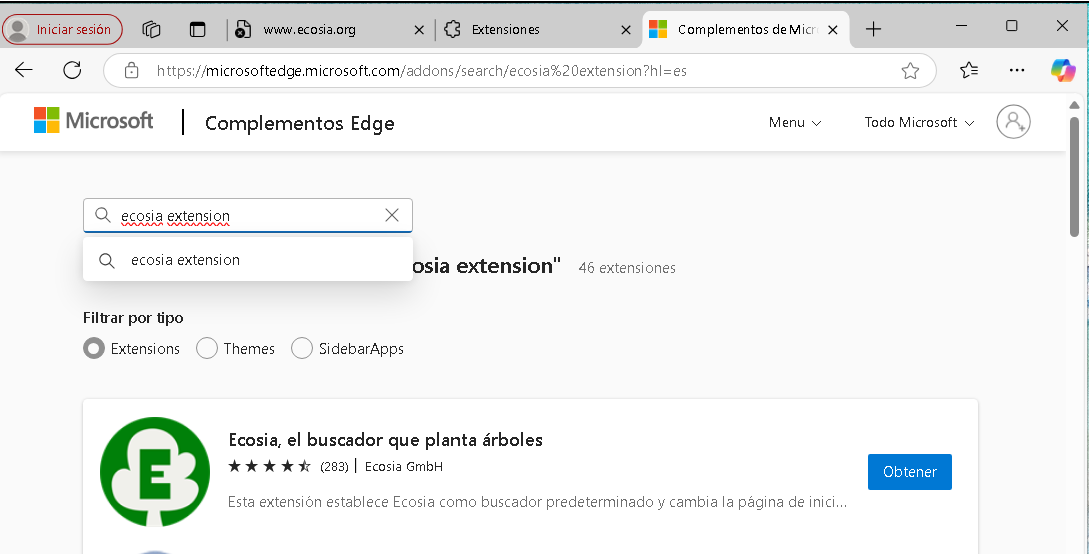
\includegraphics{png/1-EdgeExtensions.png}
\caption{\emph{Imatge 16: Instal·lem l'extensió}}
\end{figure}

\begin{center}\rule{0.5\linewidth}{0.5pt}\end{center}

\end{document}
